\section{PS2: Traingle Fractal}\label{sec:ps2}
\graphicspath{{ps2}}
\subsection{Discussion:}\label{sec:ps2:disc}
This Triangle Fractal is a variation of the Sierpinski triangle. The Polish mathematician Waclaw Sierpinski
described the pattern in 1915, but it has appeared in Italian art since the 13th century.

In this Assignment, We have to create a Triangle using only Recursion and display on the window by the help of the SFML.
We have to utilize the SFML Drawable class for the drawing of the Triangles. These traingles are similar to Sierpinski triangle but not the same. In this ps2, The triangles are created for the 3 sides of each and every triangle until unless the depth of the triangle becomes zero. The program should take two command line inputs, L and  N in that order:
\begin{itemize}
    \item L The length of the side of the base equilateral triangle (double)
    \item N The depth of the recursion (int)
\end{itemize}
\textbf{The command Line is as Follows: \newline
\colorbox{yellow}{./TFractal 200 5 } }

\subsection{Key algorithms, Data structures and OO Designs used in this Assignment:}\label{sec:ps2:kdo}
    I added Escape key to close the window as It was convenient.
    I made use of VertexArray to draw individual triangles themselves.
    The Triangle is completely draw until the depth value becomes zero.
    I added colors to the triangle.
    I Used cmath for the math functions.I added background to the triangle as you can see in the output \textbf{Figure: \ref{fig:tri}}
    \newline Changes I did: \newline
    \begin{itemize}
        \item   I made use of VertexArray for individual triangle.
\item  Implemented different Mathematic formulas.
\item  Added Background to the Triangle.
\item  Added Cpplint to target file.
\item  Used randr() rather than rand()
    \end{itemize}
    \textbf{\colorbox{lime}{Recursive method used in ftree:}} 
    \begin{lstlisting}
fTree(tris, len / 2, depth - 1, _xcen_a, ycenter_a);
fTree(tris, len / 2, depth - 1, _xcen_b, ycenter_b);
fTree(tris, len / 2, depth - 1, _xcen_c, ycenter_c);
    \end{lstlisting}
    \textbf{\colorbox{lime}{Random Color Code:}}
    \begin{lstlisting}
    int v1 = rand_r(&range) % 255;
int v2 = rand_r(&range) % 255;
int v3 = rand_r(&range) % 255;
triangle[0].position = sf::Vector2f(xvertex_a , yvertex_a);
triangle[0].color = sf::Color(v1 , v2 , v3);
triangle[1].position = sf::Vector2f(xvertex_b , yvertex_b);
triangle[1].color = sf::Color(v1 , v2 , v3);
triangle[2].position = sf::Vector2f(xvertex_c , yvertex_c);
triangle[2].color = sf::Color(v1 , v2 , v3);
triangle[3].position = triangle[0].position;
triangle[3].color = sf::Color(v1 , v2 , v3);
    \end{lstlisting}
    \newpage

\subsection{Images used:}\label{sec:ps2:img}
\begin{figure}[h]
    \centering
    
\includegraphics[width=0.5\textwidth]{ps2/backg.jpg}
    \caption{Background for the Triangle}
    \label{fig:decode}
\end{figure}


\subsection{What I accomplished :}\label{sec:ps2:accomplish}

I have accomplished the creation of the Triangle Fractal using the Recursive methods. It was really an Amazing and effective way to create patterns using recursion. I have added random colors for it to gain extra credit.

\subsection{What I already knew :}\label{sec:ps2:knew}

I already knew how to create a window and few events. I also knew how to add background to the window and set the window size. I also knew how to take command line arguments.

\subsection{What I learned :}\label{sec:ps2:learn}

I learned how to implement the sf::Drawable class in much efficient manner. I also got to know how to utilize the mathematic functions and recursive methods to draw amazing patterns.

\subsection{Challenges :}\label{sec:ps2:challenges}

To find out the exact math formula and align the triangle to the center was the challenging part.
\newpage
\subsection{Codebase}\label{sec:ps2:code}

\colorbox{pink}{\textbf{Makefile:}} \newline \textbf{This Makefile contains the linting too.}
\lstinputlisting[language=Make]{ps2/Makefile}

\colorbox{pink}{\textbf{TFractal.cpp}} \newline \textbf{This file is important as the Recursion takes place as well as the window is drawn. It calls the Triangle.cpp for creating the Triangles until unless the depth becomes zero.}
\lstinputlisting{ps2/TFractal.cpp}

\colorbox{pink}{\textbf{Triangle.h}} \newline \textbf{It is a header file where the initialization of libraries as well as variables and methods takes place.}
\lstinputlisting{ps2/Triangle.h}

\newpage

\colorbox{pink}{\textbf{Triangle.cpp}} \newline \textbf{This file utilizes the SFML library to create the Triangles.}
\lstinputlisting{ps2/Triangle.cpp}





\subsection{Output:}\label{sec:ps2:output}
\begin{figure}[h]
    \centering
    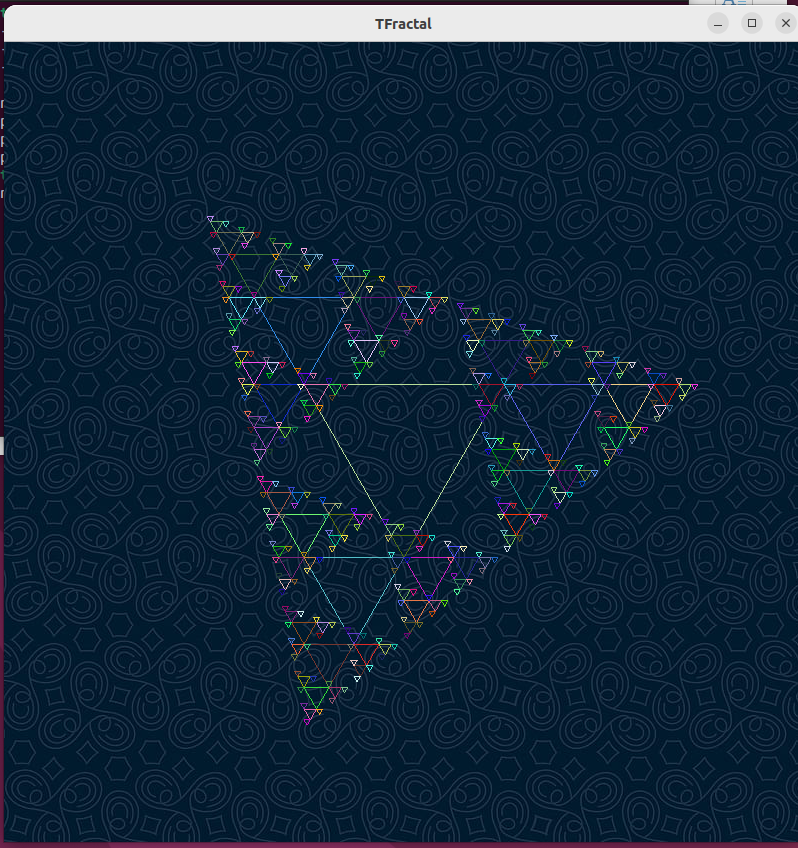
\includegraphics[width=0.7\textwidth]{ps2/screenshot.png}
    \caption{Triangle TFractal}
    \label{fig:tri}
\end{figure}

\newpage
